\documentclass[a4paper,10pt,twocolumn]{article}
\usepackage[utf8]{inputenc}
\usepackage[top=1.8cm,bottom=2.0cm,right=1.35cm,left=1.35cm,columnsep=0.5cm]{geometry}
\usepackage{setspace, url}
\usepackage[natbibapa]{apacite}
\bibliographystyle{apacite}
\usepackage{graphicx}
\usepackage{amsmath}
\usepackage{amsfonts}
\usepackage{amssymb}
\usepackage{enumitem}

\newcommand{\mbold}[1]{\boldsymbol{#1}}
\usepackage[dvipsnames]{xcolor}


\newcommand{\hilight}[2][MidnightBlue]{\textcolor{#1}{#2}}

\usepackage{lipsum}% this geenerates fictitious text for sample
%opening
\title{Intrusion detection using logistic regression: A comparison of regularization methods and PCA-logistic regression method}
\author{Karan Goel \\
        School of Computing and Information Technology\\
        University of Wollongong\\
        CSCI933, SN:7836685, \url{kg956@uowmail.edu.au}}
\date{April 19, 2024}

\begin{document}
\onehalfspacing
\twocolumn[
  \begin{@twocolumnfalse}
    \maketitle
    \begin{abstract}
This study explores the application of logistic regression to intrusion detection, framing it as a binary classification problem within the context of Internet of Things (IoT) environments. We investigate various regularization techniques—lasso, ridge, and elastic-net—to assess their effectiveness in model performance enhancement, complemented by a dimensionality reduction approach using Principal Component Analysis (PCA). Utilizing a comprehensive real-time IoT dataset, the models demonstrate high accuracy, with the best performing model, which integrates ridge regularization and the Newton-CG solver, achieving an accuracy of 98.6\%. Additionally, models employing PCA to reduce feature dimensionality also showed promising results with accuracy of 98.8\%, maintaining high accuracy while reducing computational complexity.

    \end{abstract}
  \end{@twocolumnfalse}
]

\section{Introduction}
\label{sec:introduction}
In today's digitally interconnected landscape, safeguarding computer networks against malicious activities is an imperative task. The proliferation of network devices across various sectors, including healthcare, manufacturing, and agriculture, has led to an unprecedented surge in connectivity and data exchange. However, this interconnectedness exposes networks to potential exploitation by cybercriminals, posing significant threats to data integrity and network security.

As organizations increasingly rely on digital infrastructure to streamline operations, the need for robust intrusion detection mechanisms has become paramount. In this context, integrating machine learning techniques has garnered substantial attention for their potential to enhance the efficacy of intrusion detection systems. Our study delves into machine learning-driven intrusion detection, focusing on the application of logistic regression models.

Our primary objective is to evaluate the efficiency and effectiveness of logistic regression in accurately classifying network traffic as normal or indicative of a potential attack. Additionally, we will assess the trade-offs between model complexity, interpretability, and predictive performance to determine the optimal configuration for real-world applications.

This study evaluates several logistic regression methodologies for intrusion detection, including: \textbf{1) No regularization}, using a basic model setup; \textbf{2) L2 regularization (ridge)}, which mitigates overfitting by adding a penalty term that encourages smaller parameter values, enhancing model generalization; \textbf{3) L1 regularization (lasso)}, which promotes model simplicity and feature selection by penalizing the absolute values of regression coefficients; \textbf{4) L1-L2 regularization (elastic-net)}, which combines L1 and L2 to balance sparsity and parameter shrinkage, useful for correlated features; and \textbf{5) PCA for dimensionality reduction}, which projects features onto a lower-dimensional space to enhance computational efficiency and address the curse of dimensionality.

\subsection*{Existing Works}
Numerous studies have endeavored to enhance intrusion detection systems through a variety of machine learning techniques, among them logistic regression. For example, Wang et al. \cite{wang2005multinomial} introduced an innovative ensemble approach utilizing a multinomial logistic regression model tailored to the most prevalent attack types. Similarly, Gu et al. \cite{gu2020effective} devised a method that combines partial least squares regression and logistic regression with feature augmentation to achieve comparable results.

\cite{shyla2022optimization} proposed adaptive moment estimation-stochastic gradient descent with Ridge classifier, Logistic Regression, and an ensemble method in terms of both time complexity and accuracy.

Although our study does not employ any of the aforementioned methods in the realm of intrusion detection, it's important to acknowledge the diverse approaches that have been explored in the field.

\section{Theory and properties of regression}
Regression is a statistical method by which one variable is explained or understood on the basis of one or more other variables. The variable that is being explained is called the dependent, or response, variable; the other variables used to explain or predict the response are called independent variables.
\cite{alma991003312373606666}

A regression problem involves finding a hypothesis $h$ from a set of functions mapping $X$ to $Y$, given a labeled sample $S$ where inputs are drawn from an unknown distribution $D$. The objective is to minimize the expected loss or generalization error $R(h)$ with respect to the target function $f$. The loss function $L$ measures the error between predicted and actual labels, commonly using squared error for $L(y, \hat{y}) = ||y - \hat{y}||^2$. The generalization error $R(h)$ is defined as the expected value of the loss function over the distribution $D$. The empirical loss $\hat{R}(h)$ is computed as the average loss over the labeled sample $S$. These are mathematically expressed as:

\begin{equation}
R(h) = \mathbb{E}_{x \sim D}[L(h(x), f(x))] \label{eq:generalization_error}
\end{equation}

\begin{equation}
\hat{R}(h) = \frac{1}{m} \sum_{i=1}^{m} L(h(x_i), y_i) \label{eq:empirical_loss}
\end{equation}

Here, $x_i$ and $y_i$ represent the input-output pairs in the labeled sample, and $h(x_i)$ is the predicted output by the hypothesis $h$. \cite{27578920080101}

\subsection{L1, L2 and Elastic-net penalties}
Regularization techniques such as L1, L2, and Elastic Net are widely used in machine learning and statistics to prevent overfitting and improve the generalization of predictive models.

\begin{enumerate}[label={}]
\item \textbf{L1 Regularization (Lasso Regression):}
L1 regularization adds a penalty term to the cost function equal to the absolute value of the magnitude of coefficients.

\[ J(\mathbf{w}) = \text{Cost}(\mathbf{w}) + \lambda \sum_{i=1}^{n} |\mathbf{w}_i| \]

where \( \text{Cost}(\mathbf{w}) \) is the original cost function, \( \lambda \) is the regularization parameter, and \( |\mathbf{w}_i| \) represents the absolute value of the \( i \)-th coefficient.

L1 regularization encourages sparse solutions by driving some coefficients to exactly zero. This leads to feature selection, making it effective when dealing with datasets containing many irrelevant features.  \cite{27578920080101}

\item \textbf{L2 Regularization (Ridge Regression):}
 L2 regularization adds a penalty term to the cost function equal to the squared magnitude of coefficients. 
 
 \[ J(\mathbf{w}) = \text{Cost}(\mathbf{w}) + \lambda \sum_{i=1}^{n} \mathbf{w}_i^2 \]
 
where \( \text{Cost}(\mathbf{w}) \) is the original cost function, \( \lambda \) is the regularization parameter, and \( \mathbf{w}_i^2 \) represents the squared value of the \( i \)-th coefficient.

L2 regularization penalizes large coefficients and shrinks them towards zero, but it rarely leads to zero coefficients. It helps in reducing the impact of irrelevant features and can improve the numerical stability of the solution. \cite{27578920080101}

\item \textbf{Elastic Net Regularization:}
Elastic Net combines L1 and L2 penalties by adding both penalties to the cost function.

\[ J(\mathbf{w}) = \text{Cost}(\mathbf{w}) + \lambda_1 \sum_{i=1}^{n} |\mathbf{w}_i| + \lambda_2 \sum_{i=1}^{n} \mathbf{w}_i^2 \]

where \( \text{Cost}(\mathbf{w}) \) is the original cost function, \( \lambda_1 \) and \( \lambda_2 \) are the regularization parameters for L1 and L2 penalties respectively.

Elastic Net combines the benefits of both L1 and L2 regularization. It encourages sparsity like L1 regularization while also handling multicollinearity among features like L2 regularization. The solution weight vector is modified by both penalties, resulting in a balance between feature selection and coefficient shrinkage. \cite{27578920080101}
\end{enumerate}

\subsection{Logistic regression}

In Logistic Regression, the dependent variable is binary, meaning it possesses two distinct values such as True/False, 0/1, or Yes/No. This model serves to assess the likelihood of a dichotomous outcome based on one or more independent variables. Employing the logistic function, it establishes the relationship between the dependent variable and the independent variables.

Logistic Regression shares similarities with Linear Regression, as it stands as a special case within the realm of Generalized Linear Models. However, notable disparities exist between these two methodologies. In Logistic Regression, the Conditional Distribution y|x does not conform to a Gaussian distribution but rather adheres to a Bernoulli distribution.
Predicted outcomes in Logistic Regression manifest as probabilities computed via the logistic function, constrained within the range of 0 to 1.

The outcomes derived from Logistic Regression can be expressed through the following equations:

\[
P(Y=1|X) = \frac{1}{1 + e^{-(\beta_0 + \beta_1 X_1 + \beta_2 X_2 + \ldots + \beta_n X_n)}}
\]

\[
P(Y=0|X) = 1 - P(Y=1|X)
\]

Where:
- \( P(Y=1|X) \) represents the probability of the dependent variable \( Y \) being 1 given the values of the independent variables \( X \).
- \( \beta_0, \beta_1, \beta_2, \ldots, \beta_n \) are the coefficients of the logistic regression model.
- \( X_1, X_2, \ldots, X_n \) are the independent variables.
- \( e \) is the base of the natural logarithm. \cite{alma991003312373606666}

\subsection{PCA-logistic regression}

Principal Components Analysis (PCA) is a linear technique for dimensionality reduction, which means that it performs dimensionality reduction by embedding the data into a linear subspace of lower dimensionality. Although there exist various techniques to do so, PCA is by far the most popular (unsupervised) linear technique. Therefore, in our comparison, we only include PCA.

PCA constructs a low-dimensional representation of the data that describes as much of the variance in the data as possible. This is done by finding a linear basis of reduced dimensionality for the data, in which the amount of variance in the data is maximal.

In mathematical terms, PCA attempts to find a linear mapping $M$ that maximizes the cost function $\text{trace}[M^\top \Sigma M]$, where $\Sigma$ is the covariance matrix of the data.

The covariance matrix $\Sigma$ is given by:
\[
\Sigma = \frac{1}{n} \sum_{i=1}^{n} (\mathbf{x}_i - \mathbf{\mu})(\mathbf{x}_i - \mathbf{\mu})^\top
\]
where $\mathbf{x}_i$ represents the $i$-th data point and $\mathbf{\mu}$ is the mean of the data.

\cite{maaten2009}

\section{Experiments}

In this study, we carried out the following experiments:

\begin{enumerate}
    \item \textbf{Regularization and Solver Comparison}: We Investigated the effect of different optimizer (solvers) on the performance of logistic regression models with various regularization techniques.
    \item \textbf{Feature Selection via PCA}: We Experimented with different percentages of retained features using PCA (Principal Component Analysis) and observe how it impacts the model's accuracy.
\end{enumerate}

\subsection{Internet-of-things dataset}

The RT-IoT2022 dataset provides a comprehensive collection sourced from an operational IoT infrastructure, encompassing a diverse range of IoT devices and intricate network attack scenarios. It encompasses both normal and adversarial behaviors, offering a realistic portrayal of real-world situations. The dataset features data from various IoT devices such as ThingSpeak-LED, Wipro-Bulb, and MQTT-Temp, alongside various simulated attacks. \cite{misc_rt-iot2022__942}.

For the purpose of this study, we have re-framed the dataset for a binary classification problem, relabeling all IoT device traffic as 'Normal - 0' and simulated attacks as 'Attack - 1'. A concise overview of the dataset can be observed in the Table ~\ref{tab:dov} below.

\begin{table}[h!t]
\caption{Dataset Overview}
{%
\newcommand{\mc}[3]{\multicolumn{#1}{#2}{#3}}
\begin{center}
\begin{tabular}{|c|c|}
\hline
\textbf{Dataset} & RT-IoT2022\\
\textbf{Number of Features} & 83\\
\textbf{Instances} & 123117\\
\hline
\textbf{Attack Labels (1)} & \begin{tabular}[c]{@{}c@{}}'ARP\_poisoning',\\
 'DDOS\_Slowloris', \\
 'DOS\_SYN\_Hping',\\
 'Metasploit\_Brute\_Force\_SSH',\\
 'NMAP\_FIN\_SCAN',\\
 'NMAP\_OS\_DETECTION',\\
 'NMAP\_TCP\_scan',\\
 'NMAP\_UDP\_SCAN',\\
 'NMAP\_TREE\_SCAN'\end{tabular}\\
 \hline
\textbf{Normal Labels (0)} & \begin{tabular}[c]{@{}c@{}}'MQTT\_Publish',\\
 'Thing\_Speak',\\
 'Wipro\_bulb'\end{tabular}\\
\hline
\end{tabular}
\end{center}
}%
\label{tab:dov}
\end{table}

\subsection{Experimental setup}

To ensure the robustness of the study, we have set up our experiments in four distinct stages: Data Analysis, Pipeline Setup, Training, and Inference. Each stage plays a crucial role in ensuring the reliability and validity of our experimental findings.

\subsubsection{Data Analysis}

We thoroughly explore the dataset to gain insights into its features, including their types (numerical, categorical - Table \ref{tab:dt}) and distributions. Within the given dataset, we identified two categorical features in the input space, namely "protocol" and "service". On further examination for potential biases and discrepancies in the dataset we observed a potential bias towards attack traffic, which accounted for more than half of the dataset, same bias can be observed for protocol distribution. This finding sheds light on the imbalance in the dataset, which needs to be accounted before model can be trained.

\begin{table}[h!]
\caption{Data Types of Features}
\begin{center}
\begin{tabular}{|l|l|}
\hline
\textbf{Data Type} & \textbf{Count} \\ \hline
float64 & 47 \\
int64 & 34 \\
object & 2 \\ \hline
\end{tabular}
\end{center}
\label{tab:dt}
\end{table}

\subsubsection{Data Splitting}

\begin{figure}[h!t]
    \centering
    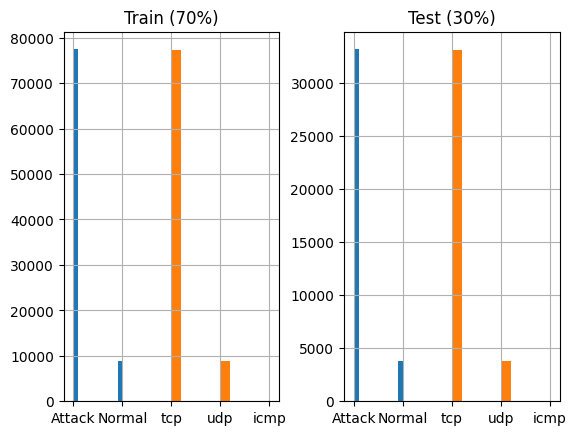
\includegraphics[scale=0.5]{split.png}%
    \caption{Train-Test Split}
    \label{fig:split}
\end{figure}

The dataset is divided into training and test sets, with the training set utilized for model training and the test set employed to assess the final model performance. To mitigate potential bias in the data distribution, we implemented a standard 70-30 split using StratifiedKFold, ensuring equal distribution of class labels across the dataset. This split strategy is illustrated in Figure~\ref{fig:split}.

\subsubsection{Pipeline Setup}

\begin{figure}[h!t]
    \centering
    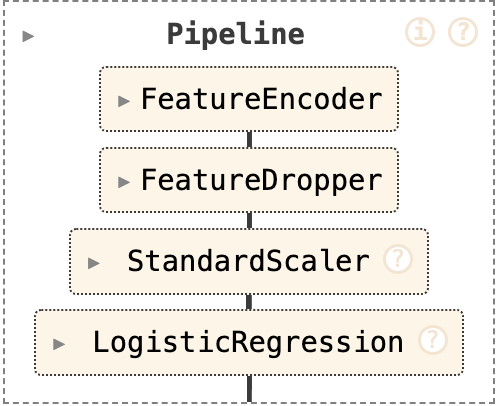
\includegraphics[scale=0.5]{pipeline.png}%
    \caption{Pipeline}
    \label{fig:pipeline}
\end{figure}

To ensure the consistency and efficiency of our experiments, we have established a systematic pipeline comprising several key steps.

\begin{enumerate}
    \item \textbf{FeatureEncoder}: Categorical features are encoded into numerical representations. We utilize a custom encoder with one-hot encoding as its base to handle categorical variables effectively.
    
    \item \textbf{FeatureDropper}: A custom feature dropper is implemented to remove redundant features such as port numbers and IDs.
    
    \item \textbf{StandardScaler}: Features are standardized using the StandardScaler, which removes the mean and scales the data to unit variance.
\end{enumerate}

\subsection{Experiment 1: Regularization and Solver Comparison}

This experiment aims to evaluate the impact of regularization techniques and compare different solvers for logistic regression models. The experiment is structured as follows:

\begin{enumerate}
    \item \textbf{Model Setup}: Multiple logistic regression models are created using our initial pipeline (Figure \ref{fig:pipeline}).
    
    \item \textbf{Regularization Techniques}: Each model's hyperparameters are fine-tuned with different penalties (None, l1, l2, elastic-net) using compatible solvers (refer to the compatibility matrix in Table \ref{solver}).
    
    \item \textbf{Performance Metrics}: Performance metrics including accuracy, precision, recall, and F1-score are computed for each model.
\end{enumerate}

\begin{table}[h!]
\caption{Solver and Regularization Pairings}
\begin{center}
\begin{tabular}{|l|c|c|c|c|}
\hline
\textbf{Penalty} & \textbf{lbfgs} & \textbf{liblinear} & \textbf{newton-cg} & \textbf{saga} \\ \hline
\textbf{None} & \checkmark & & \checkmark & \checkmark \\
\textbf{l1} & & \checkmark & & \checkmark \\
\textbf{l2} & \checkmark & \checkmark & \checkmark & \checkmark \\
\textbf{elastic-net} & & & & \checkmark \\ \hline
\end{tabular}
\label{solver}
\end{center}
\end{table}

Through this experiment, we aim to gain a deeper understanding of the role of regularization techniques in logistic regression models.

\subsection{Experiment 2: Feature Selection via PCA}

In this experiment, we investigate the impact of feature selection using Principal Component Analysis (PCA) on model performance. The experiment is structured as follows:

\begin{enumerate}
    \item \textbf{Percentage of Retained Features}: We experiment with different percentages of retained features using PCA. By varying the number of principal components retained, we observe how it affects the model's accuracy and performance.
    
    \item \textbf{Model Performance}: The performance of models trained with different percentages of retained features is evaluated using standard evaluation metrics such as accuracy, precision, recall, and F1-score.

\end{enumerate}

Through this experiment, we aim to determine the optimal number of features to retain using PCA and its impact on model performance and generalization.

\subsection{Results}

\subsubsection{Experiment 1 Result}

In the Experiment 1 results, it's notable from Table \ref{ex1res} that L2 regularization with the Newton-CG solver achieved the highest accuracy of 98.6\%. This indicates the effectiveness of this particular combination in optimizing the logistic regression model for the dataset.

Figure \ref{fig:regres} showcases the performance of each solver in terms of accuracy. This visual representation helps to illustrate how different solvers compare in terms of their ability to optimize the model's accuracy.

\begin{table}[h!]
\caption{Performance Metrics}
\begin{center}
\begin{tabular}{|c|c|c|c|c|}
\hline
\textbf{Parameters} & \textbf{Accuracy} & \textbf{Precision} & \textbf{Recall} & \textbf{F1} \\ \hline
None-lbfgs & 98.4 & 99.0 & 99.3 & 99.1 \\
None-newton & 92.3 & 92.9 & 99.0 & 95.9 \\
None-saga & 98.0 & 99.0 & 98.7 & 98.9 \\
l1-liblinear & 98.2 & 99.3 & 98.7 & 99.0 \\
l1-saga & 98.0 & 99.0 & 98.7 & 98.9 \\
l2-lbfgs & 98.4 & 99.0 & 99.2 & 99.1 \\
l2-liblinear & 98.2 & 99.1 & 98.8 & 99.0 \\
l2-newton & 98.6 & 99.4 & 99.1 & 99.2 \\
l2-saga & 98.0 & 99.0 & 98.7 & 98.9 \\
elasticnet-saga & 98.0 & 99.0 & 98.7 & 98.9 \\
\hline
\end{tabular}
\end{center}
\label{ex1res}
\end{table}

\begin{figure}[h!t]
    \centering
    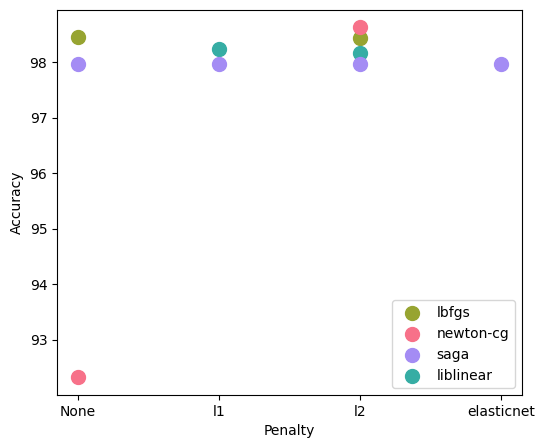
\includegraphics[scale=0.6]{res4.png}%
    \caption{Regularization and
Solver Comparison}
    \label{fig:regres}
\end{figure}

\subsubsection{Experiment 2 Result}
In Experiment 2, we systematically explored the effect of increasing the dimensionality in our PCA-transformed feature set on model accuracy. Notably, there was a progressive improvement in accuracy correlating with the number of dimensions retained. The peak accuracy reached 98.8\% when we preserved 59 dimensions, constituting about 75\% of the original feature set. This observation indicates that the PCA was effective not only in reducing the dataset's complexity but also in retaining sufficient critical information to enhance the model's predictive accuracy.

Figure \ref{fig:pca} visually depicts the relationship between the number of dimensions retained and the corresponding model accuracy, clearly illustrating the positive impact of increased dimensions up to a certain threshold on model performance.

\begin{figure}[h!t]
    \centering
    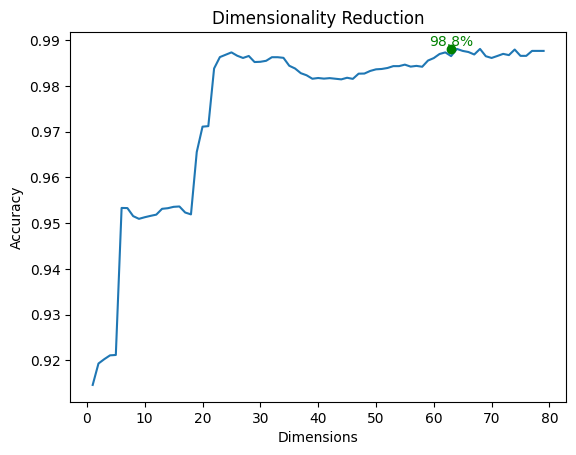
\includegraphics[scale=0.6]{pca.png}%
    \caption{PCA Result}
    \label{fig:pca}
\end{figure}

\section{Discussion}
\label{sec:discussion}

\begin{enumerate}
    \item \textbf{Effectiveness of Regularization Techniques}: 
    Our findings reveal that L2 regularization paired with the Newton-CG solver achieved the highest accuracy of 98.6\%. This underscores the efficacy of L2 regularization in managing overfitting, which is crucial in high-dimensional data environments like intrusion detection systems. L2 regularization's ability to penalize the square of coefficient values effectively constrains model complexity while maintaining predictive performance. Conversely, L1 regularization, which promotes sparsity by driving some coefficients to zero, demonstrated slightly lower performance. However, its utility in feature selection could be invaluable in scenarios where model interpretability is as critical as model performance.

    \item \textbf{Impact of PCA on Model Performance}:
    The utilization of PCA to reduce dimensionality while retaining 75\% of the original features resulted in a top accuracy of 98.8\%. This finding illustrates that PCA can condense essential information into a reduced set of features without significantly compromising the model’s accuracy. Such dimensionality reduction not only simplifies the model but also enhances computational efficiency, which is vital for real-time intrusion detection systems.

    \item \textbf{Comparison with Other Studies}:
    Comparing our approach with the methodologies employed in prior studies such as those by \cite{wang2005multinomial}  and \cite{gu2020effective}, our logistic regression models appear to offer a balance between accuracy and computational demands. Unlike the multinomial logistic regression model by Wang et al., which targets specific attack types, our binary classification approach provides a broader application potential with high accuracy across various attack scenarios.
\end{enumerate}

\subsection{Theoretical and Practical Implications}
The robust performance of logistic regression models equipped with L2 regularization and PCA highlights the robustness of these methods in cybersecurity applications, reinforcing the theoretical framework that supports logistic regression as a powerful tool for binary classification, particularly in environments as dynamic and vulnerable as IoT-based networks. Furthermore, the practical implications of our study are significant for cybersecurity professionals seeking efficient and accurate intrusion detection solutions. The demonstrated effectiveness of L2 regularization and PCA in reducing model complexity and improving prediction accuracy suggests that these techniques can be readily adopted in real-world intrusion detection systems, potentially enhancing their ability to thwart cyber-attacks.

\subsection{Limitations and Future Research}
While our results are promising, they are not without limitations. The potential biases in the RT-IoT2022 dataset and the generalizability of our findings to different network environments or attack types need further exploration. Future research could explore the integration of logistic regression with other machine learning techniques to address multi-class classification problems in intrusion detection. Additionally, examining the impact of other dimensionality reduction techniques could further enhance the applicability and effectiveness of logistic regression models in diverse cybersecurity contexts.

\section{Conclusion}
\label{sec:conclusion}

In conclusion, this study underscores the utility of logistic regression models in the field of cybersecurity, particularly for intrusion detection in IoT networks. The combination of L2 regularization and PCA not only achieves high accuracy but also maintains manageable model complexity, making it suitable for practical applications. The insights gained from this research contribute to the ongoing efforts to fortify digital infrastructures against evolving cyber threats.

\bibliography{report_template}

\end{document}
